\documentclass[12pt]{article}

\usepackage[utf8]{inputenc}
\usepackage{ucs}
\usepackage[T1]{fontenc}
\usepackage[francais]{babel}
\usepackage{xcolor}
\usepackage{listings}
\usepackage{mathptmx}
\usepackage{anyfontsize}
\usepackage{t1enc}
\usepackage[top=2cm, bottom=2cm, left=2cm, right=2cm]{geometry}
\usepackage{titlesec}
\usepackage{tikzducks}
\usepackage{titling}
\usepackage{graphicx}
\usepackage{wrapfig}
\usepackage{csquotes}
\usepackage{mdframed}
\usepackage[colorlinks = true,
            linkcolor = black,
            urlcolor  = black,
            citecolor = black,
            anchorcolor = black]{hyperref}
\usepackage[justification=centering]{caption}

\newcommand{\changeurlcolor}[1]{\hypersetup{urlcolor=#1}}

\renewcommand\maketitlehooka{\null\mbox{}\vfill}
\renewcommand\maketitlehookd{\vfill\null}

\definecolor{codegreen}{rgb}{0,0.6,0}
\definecolor{codegray}{rgb}{0.5,0.5,0.5}
\definecolor{codepurple}{rgb}{0.58,0,0.82}
\definecolor{backcolour}{rgb}{0.95,0.95,0.92}
\definecolor{codekeywords}{rgb}{0.1,0.53,0.92}
\definecolor{light-gray}{gray}{0.95}

\lstdefinestyle{c++}{
    backgroundcolor=\color{backcolour},   
    commentstyle=\color{codegreen},
    keywordstyle=\color{codekeywords},
    numberstyle=\tiny\color{codegray},
    stringstyle=\color{codepurple},
    basicstyle=\ttfamily\footnotesize,
    breakatwhitespace=false,         
    breaklines=true,                 
    captionpos=b,                    
    keepspaces=true,                 
    numbers=left,                    
    numbersep=5pt,                  
    showspaces=false,                
    showstringspaces=false,
    showtabs=false,                  
    tabsize=2,
    texcl=false,
    inputencoding=utf8x,
    extendedchars=true,
    literate=
  {á}{{\'a}}1 {é}{{\'e}}1 {í}{{\'i}}1 {ó}{{\'o}}1 {ú}{{\'u}}1
  {Á}{{\'A}}1 {É}{{\'E}}1 {Í}{{\'I}}1 {Ó}{{\'O}}1 {Ú}{{\'U}}1
  {à}{{\`a}}1 {è}{{\`e}}1 {ì}{{\`i}}1 {ò}{{\`o}}1 {ù}{{\`u}}1
  {À}{{\`A}}1 {È}{{\'E}}1 {Ì}{{\`I}}1 {Ò}{{\`O}}1 {Ù}{{\`U}}1
  {ä}{{\"a}}1 {ë}{{\"e}}1 {ï}{{\"i}}1 {ö}{{\"o}}1 {ü}{{\"u}}1
  {Ä}{{\"A}}1 {Ë}{{\"E}}1 {Ï}{{\"I}}1 {Ö}{{\"O}}1 {Ü}{{\"U}}1
  {â}{{\^a}}1 {ê}{{\^e}}1 {î}{{\^i}}1 {ô}{{\^o}}1 {û}{{\^u}}1
  {Â}{{\^A}}1 {Ê}{{\^E}}1 {Î}{{\^I}}1 {Ô}{{\^O}}1 {Û}{{\^U}}1
  {œ}{{\oe}}1 {Œ}{{\OE}}1 {æ}{{\ae}}1 {Æ}{{\AE}}1 {ß}{{\ss}}1
  {ç}{{\c c}}1 {Ç}{{\c C}}1 {ø}{{\o}}1 {å}{{\r a}}1 {Å}{{\r A}}1
  {€}{{\EUR}}1 {£}{{\pounds}}1
}
\lstset{style=c++}


\title{Ouai}
\author{Arquillière Mathieu - Zangla Jérémy}
\date{\today}

% \begin{lstlisting}[style=c++]
% \end{lstlisting}
% \changeurlcolor{blue}\href{run:../Documentation/latex/refman.pdf}{Lien vers la documentation Doxygen}

\begin{document}

\begin{titlepage}
  \maketitle
\end{titlepage}

\tableofcontents
\listoffigures

\newpage
\section{Lexique}

\underline{GPS} : \emph{Global Positioning System}, système de géolocalisation mondiale par satellite.

\vspace{10pt}
\underline{Smartphone} : \emph{Téléphone intelligent}, un téléphone mobile doté de fonctionnalités similaires
à un ordinateur (internet, vidéos, musiques, jeux) et de capteurs (gyroscope, GPS).

\vspace{10pt}
\underline{Application mobile} : Logiciel développé pour des supports semblables à des smartphones.

\vspace{10pt}
\underline{Serveur} : Service décentralisé permettant à des clients l'accès à des services ou des données.

\vspace{10pt}
\underline{Base de données} : Ensemble d'informations structurées accessible via un service.

\vspace{10pt}
\underline{Java} : Langage informatique.

\vspace{10pt}
\underline{Kotlin} : Langage informatique.

\vspace{10pt}
\underline{XML} : Langage informatique de structuration de données par balises.

\vspace{10pt}
\underline{Android} : Système d'exploitation créé par \emph{Google}, le plus souvent déployé sur des smartphones.

\vspace{10pt}
\underline{Processus (informatique)} : Programme en cours d'exécution sur un système.

\vspace{10pt}
\underline{Activité} : Composante métier d'une application android.

\vspace{10pt}
\underline{Fragment} : Activité liée à seulement une partie de l'écran.

\vspace{10pt}
\underline{Google Map} : Carte électronique de \emph{Google}

\vspace{10pt}
\underline{Marker} : Affichage d'une position sur une Google Map.

\vspace{10pt}
\underline{Polyline} : Affichage d'un ensemble de traits sur une Google Map.


\newpage
\section{Introduction}

L'outil numérique a envahi progressivement toutes les sphères de notre vie quotidienne. Cet outil nous semble de
plus en plus indispensable et c'est tout naturellement que, pratiquant une activité de vélo tout terrain en forêt,
nous avons souhaité developper une application en lien.

En effet, en explorant différents chemins on souhaite pouvoir s'en souvenir et les réemprunter. Le projet serait de
proposer la possibilité de repérer, baliser et répertorier ces chemins, puis de les partager avec une communauté
amateur de cyclisme.

Notre problématique est donc de répondre à ce besoin en prenant en compte les restrictions liées au sport. La
solution doit être portable, utilisable pour un cycliste. Elle doit utiliser la géolocalisation et une base de données.

Le smartphone est un support qui convient parfaitement, muni le plus souvent d'un GPS, d'une connexion internet
et d'une taille permettant d'être transporté en vélo.

Notre projet se déroule dans le cadre d'un projet de deuxième année d'école d'ingénieurs en informatique à ISIMA. C'est
dans ce contexte que nous proposons une solution.

Nous verrons tout d'abord dans ce rapport notre démarche pour analyser la problèmatique, puis ce que nous avons mis
en oeuvre pour développer une solution et enfin quel est le résultat produit et ses possibles améliorations.
\newpage
Nous tenons à remercier toutes les personnes qui nous ont aidés dans ce projet :

\vspace{10pt}
\textbf{M. Bruno Guillon}, notre tuteur de projet qui a toujours été présent pour nous conseiller et nous aider, notemment sur les problèmes de VPN
rencontrés.

\vspace{10pt}
\textbf{L'ensemble de l'équipe du Centre de Ressources Informatiques} qui s'est montrée compréhensive et patiente face à nos problèmes liés à leur
services.

\vspace{10pt}
\textbf{Nos camarades du local Isilab}, qui nous ont aidés au diagnostic du problème de VPN.

\vspace{10pt}
\textbf{Mme. Murielle Mouzat}, pour son très utile livret de consignes pour le rapport de projet.
\newpage
\newpage
\newpage
\subsection{Les outils}
\subsubsection{Machine virtuelle}
Concernant la partie serveur, nous avons demandé un support pour héberger la base de données. L'ISIMA nous a donné en conséquence un machine
virtuelle sur leurs serveurs. Pour travailler dessus, nous utilisons le \emph{ssh}. Le système d'exploitation installé est \emph{CentOS}.
Pour le savoir il faut lire le contenu du fichier \emph{/proc/version} :
\begin{mdframed}[backgroundcolor=light-gray, roundcorner=20pt,
    leftmargin=0, rightmargin=0, 
    innerleftmargin=20, linecolor=darkgray]
    Linux version 3.10.0-1062.4.3.el7.x86\_64 (mockbuild\@kbuilder.bsys.centos.org) (gcc version 4.8.5 20150623 (Red Hat 4.8.5-39) (GCC) ) \#1 SMP Wed Nov 13 23:58:53 UTC 2019
\end{mdframed}

Cela nous permet de savoir comment installer les programmes dont nous auront besoin. En effet pour utiliser et construire notre base de données
et notre serveur il nous faut quelques outils qu'on installe avec le gestionnaire de paquets de CentOS \emph{yum} :
\begin{lstlisting}[language=bash]
sudo yum install java-1.8.0-openjdk
sudo yum install mysql-server
sudo yum install screen
sudo yum install nc
sudo yum install nmap
\end{lstlisting}

Pour installer le \emph{Système de Gestion de Base de Données}. Il faut tout d'abord mettre un mot de passe administrateur
pour s'y connecter.
\begin{lstlisting}[language=bash]
sudo mysqladmin variables -u root -p
\end{lstlisting}
On peut ensuite modifier le contenu du SGBD en utilisant l'interpréteur de commandes mysql :
\begin{lstlisting}[language=bash]
MySQL -u root -p
\end{lstlisting}
Il faut enfin créer et sélectionner la base de données que l'on veut utiliser :
\begin{lstlisting}[language=bash]
CREATE DATABASE <nom de la base de données>
USE DATABASE <nom de la base de données>
\end{lstlisting}


\subsubsection{Serveur Java}

Pour l'exécution du serveur java, on utilisera Screen.
Screen est un logiciel qui permet de créer des terminaux (appelés \emph{sessions}), de s'y déconnecter puis reconnecter autant que désiré.
Ces terminaux continueront leur exécution en arrière plan. On peut donc utiliser l'entrée et la sortie standard pour communiquer avec le programme.
Pour se connecter à une session ou la créer si elle n'existe pas, on utilise l'option -R.
\begin{lstlisting}[language=bash]
    screen -R <nom_du_terminal>
\end{lstlisting}

\subsection{Base de données}
Le base de données est composée de cinq tables. La table centrale \emph{Projets} contient un identifiant unique pour le projet ainsi que les informations basiques (nom, type et date).
Une autre table \emph{Utilisateurs} se charge de contenir les informations de connexion de chaque utilisateur de l'application. Ces deux tables sont mises en relation par la table \emph{Accès} qui permet de restreindre la visibilité des projets.
Enfin il y a deux tables contenant les points. Chaque point possède des coordonnées spatiales, ainsi que l'identifiant du projets auquel il est rattaché. La seule différence entre les deux tables de points et la présence d'une coordonnée supplémentaire liée au temps. En effet un projet n'a pas besoin de dater chaque point.
\begin{figure}[ht]
    \label{Schéma de la base de données}
    \centering
    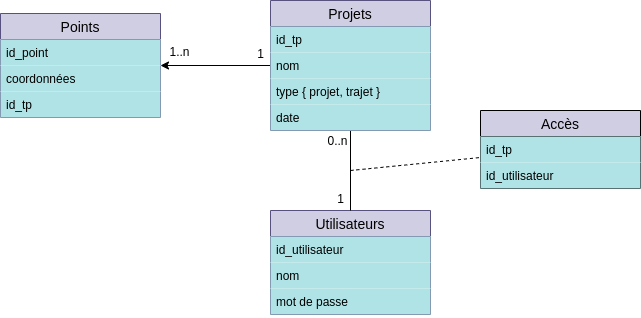
\includegraphics[scale=0.6]{images/bdd.png}
    \caption{Schéma simplifié de la base de données}
\end{figure}

\subsection{Serveur}
\subsubsection{Processus}
Le serveur utilise une architecture avec plusieurs processus. Le processus principal attend une connexion provenant d'un client (application).
A chaque connexion un nouveau processus est créé pour intéragir avec le client. Ce processus attend donc un message du client, exécute la commande
SQL nécessaire pour obtenir une réponse et répond au client en formatant les données. Un processus supplémentaire existe pour pouvoir
travailler directement avec le serveur, sans passer par un client. Pour cela, l'entrée et la sortie standard sont utilisées et il faut donc un accès direct à la machine.
\subsubsection{Classes}
Le processus principal n'utilise qu'une seule classe \emph{Serveur}, tout comme le processus de communication direct \emph{LocalCommand}.
Cependant le processus de communication avec le client est séparé en plusieurs objets : \emph{Client}, \emph{SQLHandler} et \emph{CommunicationHandler}. 
Le premier est le processus en lui même et utilise les deux autres pour effectuer les tâches qui lui sont assignées. L'objet \emph{SQLHandler} accède à la base de données et formate les réponses.
Enfin le \emph{CommunicationHandler} gère la communication réseau avec le client, il permet la réception et l'envoi de chaîne de caractères.
Enfin deux classes sont utilisées pour faciliter le travail de conversion des formats pour les points : \emph{Point3D} et \emph{Point4D} qui correspondent respectivement à une coordonnée dans l'espace : (x, y, z)
et à une coordonnée dans l'espace et le temps : (x, y, z, t).

\subsubsection{Implémentation}
La création du serveur devait à l'origine être rapide car on le considérait comme étant annexe. C'est pourquoi on a choisi l'utilisation d'une
technologie que nous connaissions déjà : \emph{Java}. Ce langage contient dans sa bibliothèque standard tout ce qu'il faut pour développer un serveur.
De plus il existe une bibliothèque Java développée par Oracle pour la communication avec les bases de données MySQL.

Le \emph{Java} est un langage compilé particulier. Le code est tout d'abord compilé dans un langage intermédiaire appelé \emph{Bytecode}. 
Puis, il est exécuté dans une machine virtuelle appelée la \emph {Java Virtual Machine} en utilisant une nouvelle étape de compilation \emph {Just In Time}.
\par
\begin{figure}[ht]
    \label{Schéma compilation Java}
    \centering
    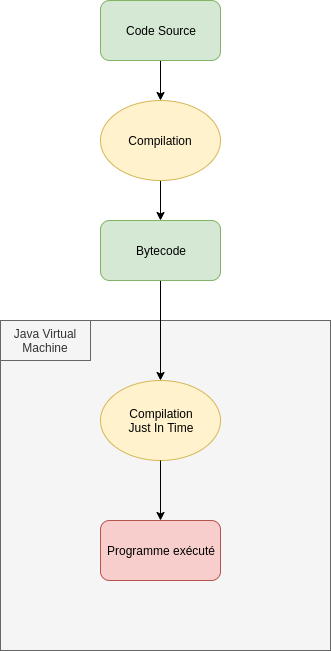
\includegraphics[scale=0.5]{images/java_compilation.png}
    \caption{Schéma représentant la compilation en Java}
\end{figure}
Les programmes développés et compilés en Java peuvent être exécutés sur toutes les machines possédant la JVM installée sans avoir aucun changement de code source ou bien de paramètre de compilation.
\subsubsection{Fonctionnement des processus}
L'organisation des processus en java est particulière. En effet, il n'y a qu'un seul processus lourd (à la différence des \emph{forks} du langage C).
Ce processus lourd unique est la JVM. Tous les autres processus, y compris le processus principal de notre programme, ne sont que des processus légers.
Il y a donc un partage des ressources, et l'échange de données est plus simple. Cependant, il faut faire attention aux accès simultanés aux ressources.
\subsubsection{Création de processus}
Le processus principal de notre programme est créé automatiquement par la JVM et il exécute le code de la fonction \emph{public static void main(String[] args)} qui est le point d'entrée de notre programme.
Pour construire d'autres processus, il y a plusieurs manières. On va ici se concentrer sur la classe \emph{Thread} et l'interface \emph{Runnable}.
\subsubsection{Utilisation de \emph{Thread}}
Un \emph{Thread} est un objet qui exécute du code dans un autre processus. Pour cela, il suffit de créer un Thread et de le lancer en utilisant la méthode \emph{start()}.
\begin{lstlisting}[language=Java]
Thread monThread = new Thread();
monThread.start();
\end{lstlisting}

Pour changer le code exécuté, il suffit de redéfinir la méthode \emph{void run()} de Thread.
\begin{lstlisting}[language=Java]
Thread monThread = new Thread() {
	@Override
	public void run() {
		System.out.println("Nouveau processus");
	}
}
monThread.start();
\end{lstlisting}

\subsubsection{Communication réseau}
En Java, on utilise les objets de type \emph{Socket} pour faire de la communication en réseau. Ces objets utilisent le protocole TCP pour communiquer et permettent donc de s'assurer de l'état de la connexion.
Un premier \emph{socket} (\emph{ServerSocket}) permet d'attendre qu'un client se connecte et de créer un \emph{Socket} pour communiquer avec lui.
\begin{lstlisting}[language=Java]
ServerSocket socket = new ServerSocket(PORT);
while (true) {
	Socket clientSocket = socket.accept();
}
\end{lstlisting}

Ensuite pour échanger avec le client, on utilise les flux d'entrée et de sortie fournis par le Socket.
Les \emph{BufferedReader} et \emph{PrintWriter} sont des objets qui permettent de traiter les flux plus simplement, grâce à des chaînes de caractères.

\begin{lstlisting}[language=Java]
InputStream input = socket.getInputStream();
OutputStream output = socket.getOutputSteam();

BufferedReader rd = new BufferedReader(new InputStreamReader(input));
PrintWriter wr = new PrintWriter(output);
\end{lstlisting}

\subsubsection{Protocole de communication}
    \begin{center}
        Liste des messages possibles dans le sens clients $\rightarrow$ serveur
        \par
        \begin{tabular}{|l|l|}
            \hline
            Commande & Utilisation\\
            \hline
            Subscribe:$<id>:<mdp>$ & Permet de s'inscrire\\
            \hline
            Connect:$<id>:<mdp>$ & Permet de se connecter à son compte\\
            \hline
            \hline
            History:$<debut>:<fin>$ & Permet de récupérer $x$ trajets entre début et fin (en id)\\
            \hline
            Projects:$<debut>:<fin>$ & Permet de récupérer les $x$ projets entre début et fin\\
            \hline
            \hline
            NewP:$<nom>:<x+y+z;...>$ & Ajoute un nouveau projet\\
            \hline
            NewJ:$<nom>:<x+y+z+t;...>$ & Ajoute un nouveau trajet\\
            \hline
            EditP:$<id>:<x+y+z;...>$ & Modifie un projet\\
            \hline
        \end{tabular}
        \addcontentsline{lot}{table}{Protocole de communication client $\rightarrow$ serveur}
    \end{center}
    \begin{center}
        Liste des messages possibles dans le sens serveur $\rightarrow$ client
        \par
        \begin{tabular}{|l|l|}
            \hline
            Commande & Utilisation\\
            \hline
            Subscribed:$<id>$ & Confirme l'inscription \\
            \hline
            Unsubscribed & Erreur lors de l'inscripton \\
            \hline
            Connected:$<id>$ & Valide la connexion à son compte\\
            \hline
            Unconnected & Erreur lors de la connection \\
            \hline
            \hline
            Project:$<id>:<nom>:<x+y+z;...;x+y+z>$ & Envoie des informations sur un projet\\
            \hline
            Journey:$<id>:<nom>:<d>:<x+y+z+t...>$ & Envoie des informations sur un projet\\
            \hline
        \end{tabular}
        \addcontentsline{lot}{table}{Protocole de communication serveur $\rightarrow$ client}
    \end{center}

  \subsubsection{Echange type}
  Lors d'un échange standard, comme celui décrit par le diagramme ci-dessous, l'utilisateur doit une fois (unique) s'inscrire via un échange \emph{Subscribe}. Le serveur lui répond en validant son inscription.
  Ensuite à chaque nouvel connexion à son compte un échange \emph{Connect} aura lieu. Ensuite la connexion sera confirmée et l'utilisateur pourra accéder aux autres fonctionnalités comme ici : la récupération des informations de son historique de trajets.
  \begin{figure}[ht]
    \label{Diagramme}
    \centering
    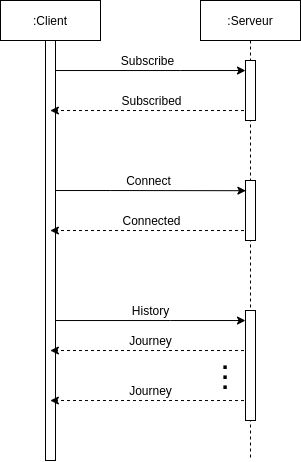
\includegraphics[scale=0.8]{images/protocole.png}
    \caption{Diagramme de séquence d'un échange entre l'application et le serveur}
  \end{figure}

\newpage
\subsection{Développement de l'application Android}
\subsubsection{Squelette de l'application}
Afin de comprendre les mécanismes du développement mobile, la première phase a été de simplement créer une application très basique, contenant
uniquement les différentes sections qu'on voudrait développer par la suite, sans leur contenu. Il a donc fallu comprendre le système des 
"activités" et des "fragments" qu'utilise Android.
\begin{itemize}
  \item Une activité est une composante métier d'une application Android et possède une "View" (un partie graphique).
  \item Un fragment s'apparente grandement à une activité. La différence est qu'un fragment est lié à une partie d'écran et non pas à un écran entier. 
\end{itemize}
Ainsi pour créer les différents onglets, on utilise une activité principale qui contient la barre d'outils  en haut avec le nom de l'onglet
dans lequel on se trouve et le bouton permettant d'afficher le menu de navigation. Ce menu est également contenu dans l'activité principale.
Chaque élément de ce menu change le fragment situé en dessous de la barre d'outils. On a donc un fragment pour chaque onglet. 
\begin{figure}[ht]
  \label{Activité-Fragment}
  \centering
  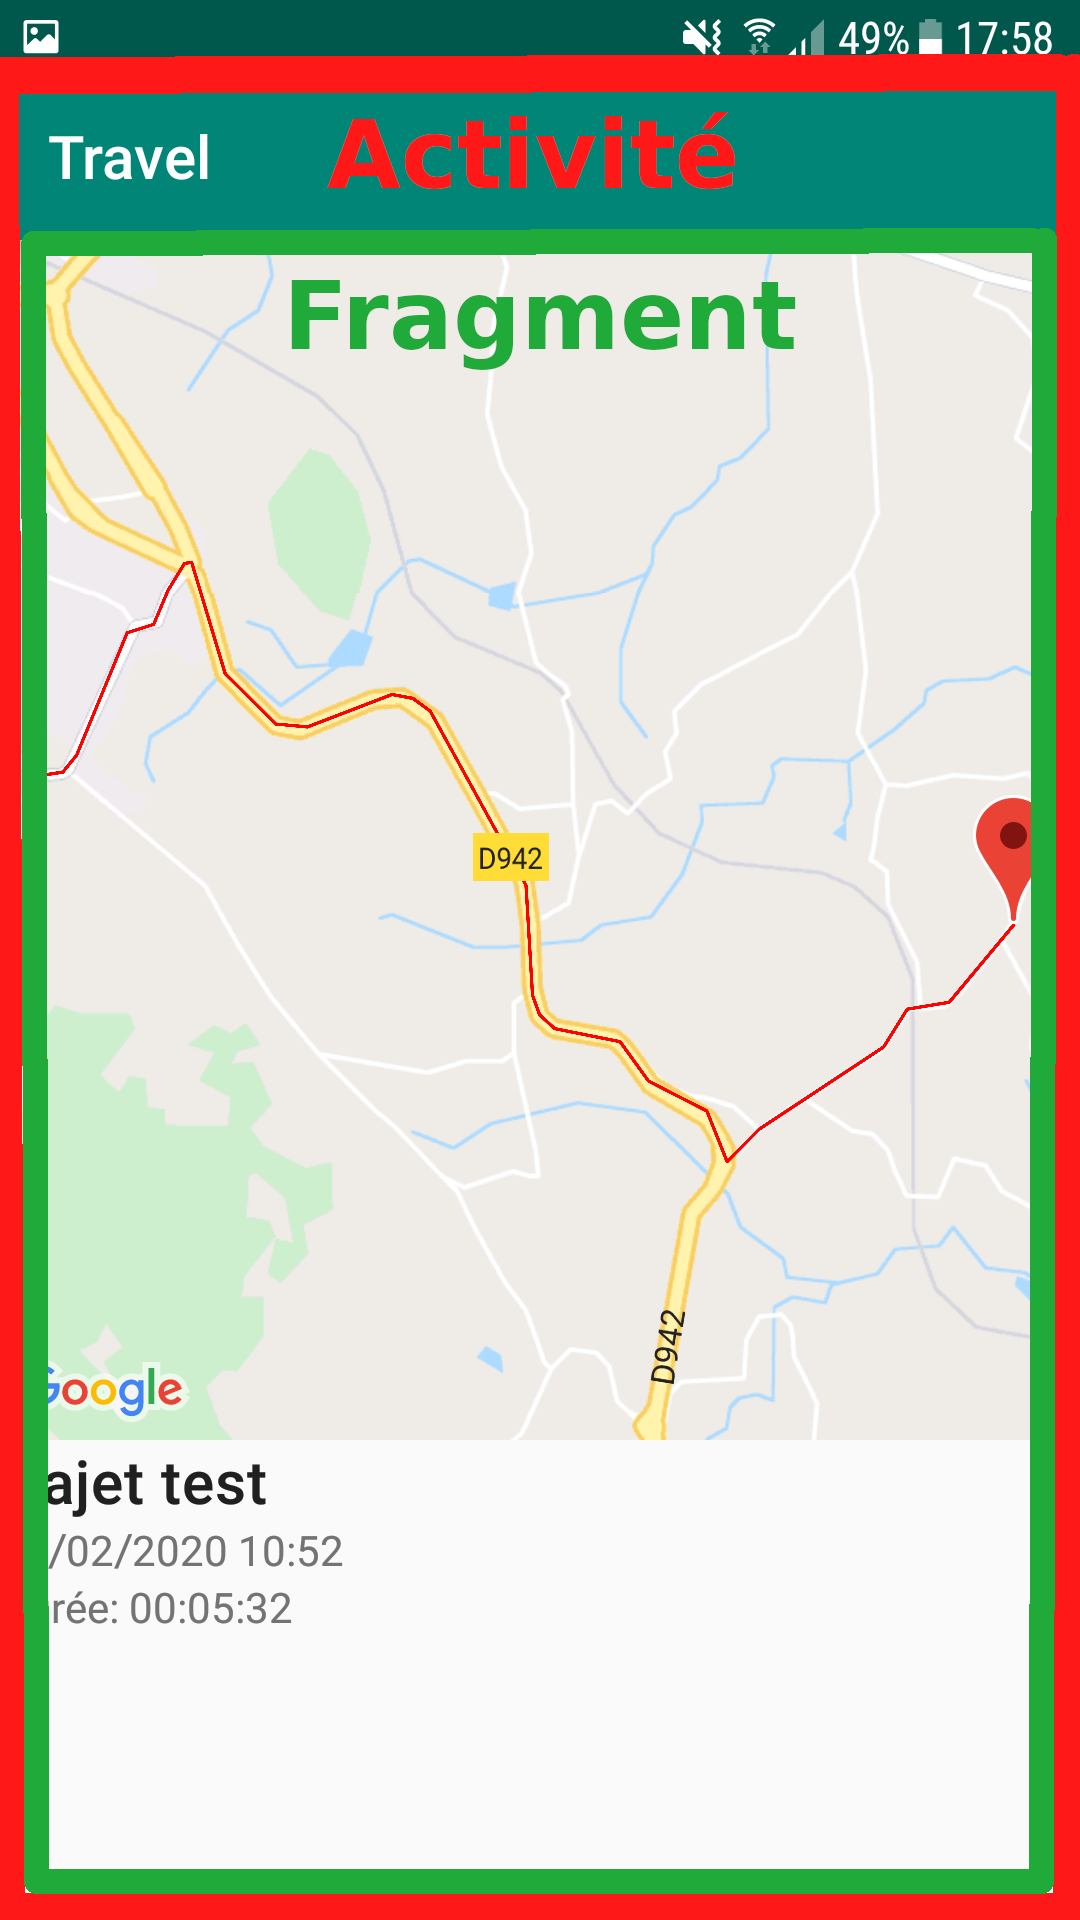
\includegraphics[scale=0.13]{images/activity-fragment.png}
  \caption{Schéma de l'imbrication d'un fragment dans l'activité principale}
\end{figure}

\subsubsection{Création d'un trajet}
Une fois plus à l'aise avec Android Studio, notre objectif premier était de pouvoir créer un simple trajet. Pour ce faire, on a utilisé un
fragment qu'on affiche lorsqu'on clique sur l'onglet "Nouveau trajet". Dans ce fragment, on a placé deux objets : une carte et un bouton.
Android Studio met à disposition des éléments complexes déjà faits et nous permet de les utiliser à travers de multiples fonctions. C'est le
cas pour les boutons et la carte électronique qui est une "Google Map". Ces éléments, que l'on place statiquement grâce au langage XML, sont
ensuite accessibles dans le code Java avec leur identifiant. On utilise ces objets en récupérant leurs informations
(par exemple quand le bouton est cliqué) ou en chageant leur apparence (par exemple en changeant le texte du bouton ou en ajoutant un trait
sur la carte).
La première étape a donc été de prendre en main les fonctionnalités d'une Google Map. Celles qui nous ont servi pour ce projet sont :
\begin{itemize}
  \item Le placement de la caméra (position et zoom)
  \item Les \emph{Markers}, qui permettent de pointer sur une position précises
  \item La \emph{Polyline}, un outil qui permet de dessiner sur la carte avec une suite de positions
\end{itemize}
Le point suivant a été de comprendre le fonctionnement d'Android pour obtenir la localisation géographique du téléphone. Le GPS n'est pas le
seul moyen d'obtenir une position. En effet il existe trois façons d'obtenir une localisation :
\begin{enumerate}
  \item le \emph{GPS\_PROVIDER} (Global Positionning System) utilise les satellites
  \item le \emph{NETWORK\_PROVIDER} utilise les wifis et le antennes téléphoniques que détecte le télephone
  \item le \emph{PASSIVE\_PROVIDER} reçoit les positions passivement lorsque d'autres applications en font la demande
\end{enumerate}
Le \emph{NETWORK\_PROVIDER} et le \emph{PASSIVE\_PROVIDER} ne donnent qu'une localisation globale, peu précise, en se servant de wifis
et d'antennes. Dans notre cas, l'utilisateur sera potentiellement éloigné de ce genre d'appareil. De plus, pour tracer un chemin réalisé
en vélo, il faut priviligier la précision des positions. Ainsi nous avons utilisé essentiellement le \emph{GPS\_PROVIDER}.

Ainsi la création d'un trajet se fait de la manière suivante :
\begin{enumerate}
  \item On clique sur l'onglet "Nouveau trajet" qui fait apparaître le fragment contenant une carte Google et un bouton "Nouveau trajet".
  Si l'application est lancée pour la première fois, une fenêtre contextuelle nous indique qu'il faut autoriser l'application à utiliser le GPS.
  Cette fenêtre permet d'ouvrir les paramètres du smartphone.
  \item On clique sur le bouton "Nouveau trajet". A ce moment l'application prend la localisation acutelle comme point de départ et fait
  apparaître un point sur la carte à cet endroit. De plus, la carte se grossit et se centre autour de ce point avec une vision d'une centaine de mètres de rayon. Le texte du bouton change et devient "Arrêter le trajet".
  \item On se déplace. Lorsque le GPS détecte un changement de position, l'application créer un nouveau point dans le trajet. Le \emph{Marker}
  se déplace sur cette nouvelle position et un trait se dessine entre le précédent point et le nouveau.
  \item On clique sur le bouton "Arrêter le trajet". Un fenêtre contextuelle permettant de rentrer le nom du trajet apparaît.
  \item On rentre le nom du trajet dans la zone de texte.
  \item On clique sur le bouton "Valider". Le trajet est créé et on peut recommencer.
\end{enumerate}
\vspace{10pt}

Avec cette première version de la création d'un trajet, il a fallu tester pour se rendre compte sur un vrai trajet si l'application était
assez précise. Pour réaliser des tests, le problème est l'utilisation du GPS, puisque contrairement à ce dont on a l'habitude de développer,
ici l'utilisateur bouge pour utiliser l'application. Il devient donc difficile de tester et corriger de manière répétée puisqu'il faut bouger
un minimum pour observer les changement du GPS, puis revenir sur son poste de travail pour corriger le problème éventuel et remettre
l'application sur le téléphone.

Cependant il existe d'autres manières de tester les applications mobiles. Par exemple Android Studio propose
un smartphone virtuel qu'on crée sur notre poste de travail afin de le manipuler et faire des tests. Pour la partie GPS, on peut injecter
à cette machine virtuelle de fausses coordonnées. Le problème lié à cette méthode est que la virtualisation d'un smartphone coûte très cher
en ressources. Ainsi Android Studio en plus de la machine virtuelle demandent un ordinateur puissant.

On peut également émuler les coordonnées GPS sur un smartphone réel grâce à des applications (disponibles sur le marché \emph{Play Store}).
On indique quelles doivent être nos coordonnées et notre GPS fait comme si il y était. Le problème soulevé par cette émulation, que ce soit
sur une machine virtuelle ou avec une application sur un smartphone, est que ça ne prend pas en compte les erreurs de positionnement GPS.
En effet lors d'un test réel, on a pu observer que le tracé du trajet se fait bien mais que par moment le GPS indique des positions fausses,
ce qui a pour effet de tracer deux traits entre ce point et le chemin qu'on parcourt. Pour pallier à ce problème, la solution pourrait être
de capturer la vitesse que nous fournit le GPS et calculer si le nouveau point qu'on veut ajouter au tracé est atteignable avec cette vitesse.
Cependant la vitesse communiquée n'est pas fiable lorsqu'on bouge lentement. On a donc décidé de faire ce traitement avec une vitesse maximale,
assez haute pour ne pas être atteinte par un cycliste.
\begin{figure}[ht]
    \label{Différence entre avant et après correction}
    \centering
    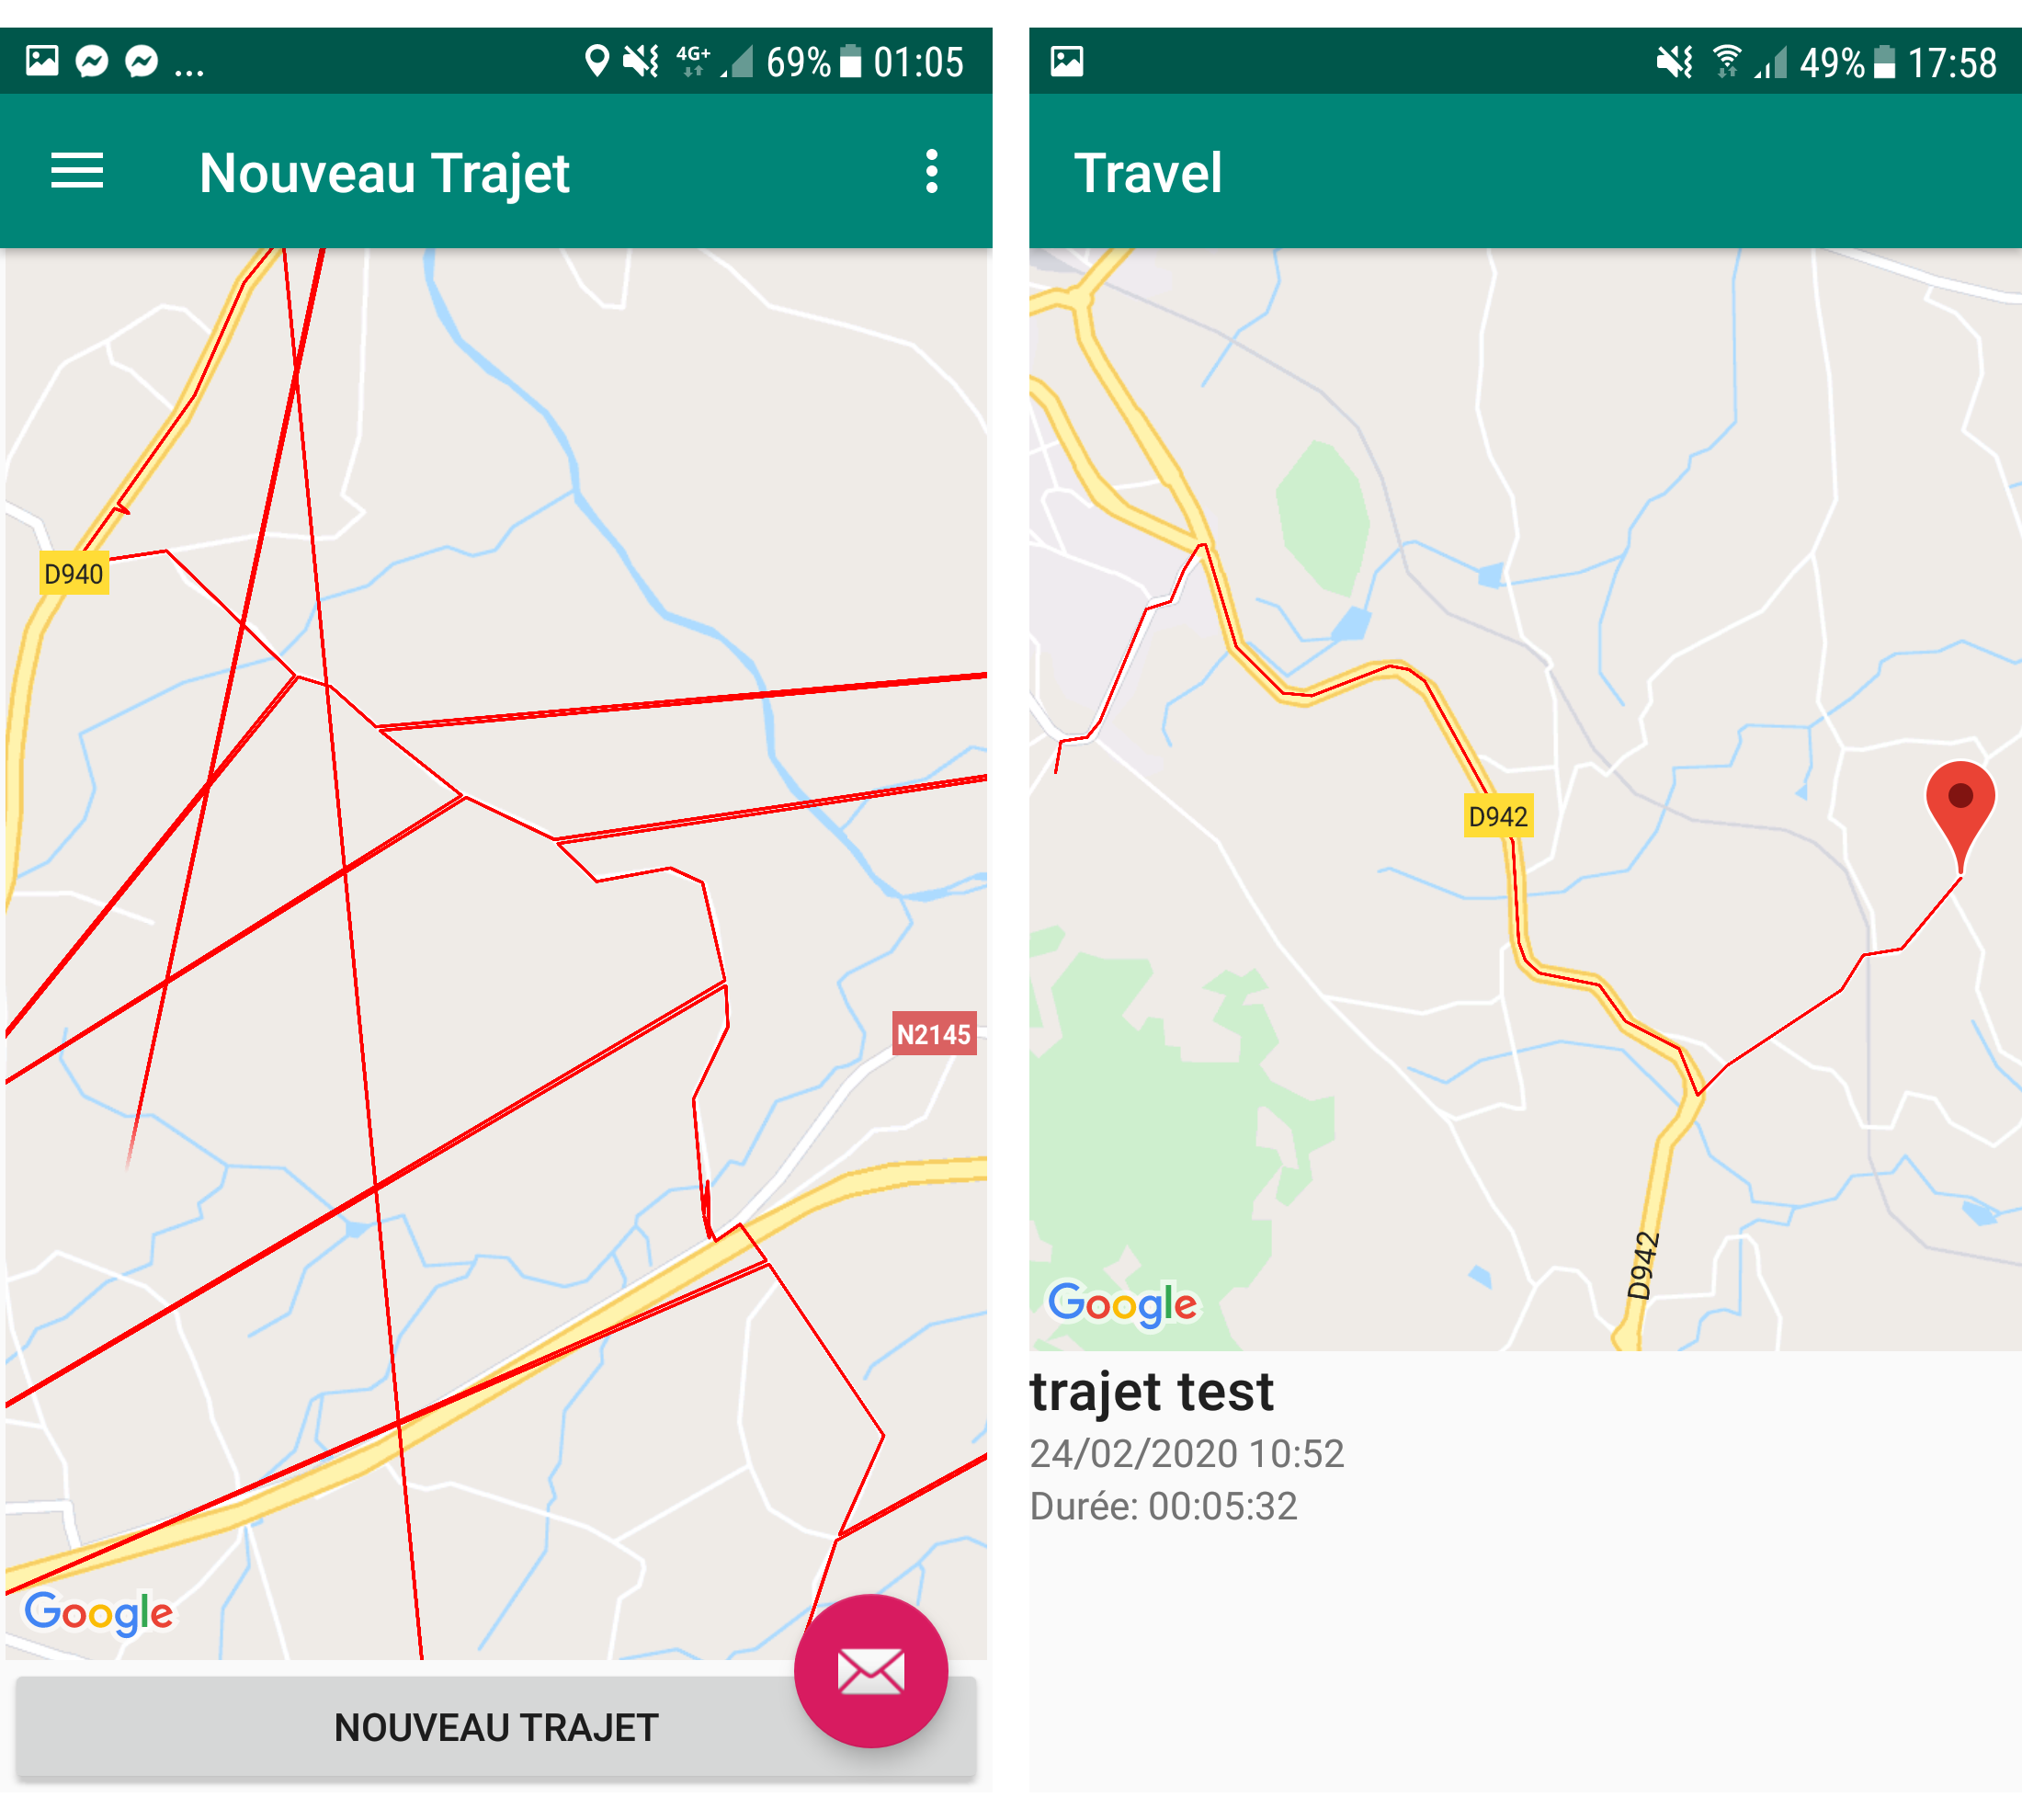
\includegraphics[scale=0.6]{images/avant-apres.png}
    \caption{Différence entre un trajet avec le problème d'imprécision du GPS et un trajet avec la correction apportée}
\end{figure}

\subsubsection{Sauvegarde des trajets}
Au début du projet, les trajets effectués par l'utilisateur étaient destinés à être enregistrés dans une base de données. Ainsi, les utilisateurs
pouvaient utiliser plusieurs appareils sans perdre leurs trajets et cela aurait permis plus tard le partage de ceux-ci. Cependant, après avoir
rencontré certains problèmes pour relier l'application smartphone au serveur, il a été décidé de sauvegarder les trajets dans des fichiers,
au moins temporairement.

Pour simplifier la communication potentielle avec le serveur, une bibliothèque Java a été réalisée pour représenter un trajet. Cette bibliothèque
contient deux objets essentiels \emph{Journey} et \emph{JourneyHistory}. L'un représentant un trajet et l'autre un ensemble de trajets
(utilisé plus tard pour l'historique). L'objet trajet n'est qu'une abstraction d'un tableau de localisations. Ces localisations possèdent
quatres composantes :
\begin{itemize}
  \item la latitude de la position
  \item la longitude de la position
  \item l'altitude de la position (pour le dénivelé du trajet)
  \item la date à laquelle le point a été pris
\end{itemize}
Ainsi à chaque nouveau point lors d'un trajet, c'est dans cet objet qu'on le stocke. Puis lorsque l'utilisateur finit son trajet,
on l'ajoute à l'objet \emph{JourneyHistory} et on écrit dans un fichier le contenu de l'objet (son nom, sa date de création et chaque
point qu'il contient).

\subsubsection{Historique}
L'objet \emph{JourneyHistory} contient en mémoire tous les trajets effectués par l'utilisateur tant que l'application est en fonctionnement.
Ainsi, lorsque l'application se démarre, on charge dans cet objet tous les trajets sauvegardés dans des fichiers. De cette manière, on peut
afficher le contenu de l'onglet "Historique" sans lire des fichiers à chaque fois.

L'affichage de cet onglet se fait via des "MaterialCards". Google met à disposition un certain nombre de composants préfaits. Ceux-ci sont
plus "design" et permettent de garder un visuel cohérent simplement. Ici nous avons utilisé les "Cards" qui sont des conteneurs pour d'autres
objets comme des images ou du texte. On ajoute simplement dans ce conteneur les éléments qui le compose et la mise en forme se fait quasi
automatiquement.

Dans l'historique, chaque "Card" représente un trajet. Une "Card" est composée d'une capture d'écran de la carte prise à la fin du trajet,
du nom du trajet, de sa date de création et de sa durée. Ainsi, lorsqu'on affiche le fragment "Historique", on crée une "Card" pour
chaque trajet dans le \emph{JourneyHistory}. Ceux-ci sont triés par date de création, on les affiche donc du plus récent au plus vieux.

Afin de pouvoir consulter les trajets de manière plus précise, le dernière fonctionnalité ajoutée a été de pouvoir cliquer sur chaque "Card"
de l'historique. Cela a pour effet d'amener vers une autre page, une autre activité permettant de consulter un trajet. Cette page contient
une Google Map avec le trajet dessiné dessus. En dessous on retrouve le nom, la date et la durée du trajet. A l'origine, cette page devait
être plus complète, avec par exemple le dénivelé du trajet, la météo ou des statistiques. De plus la carte affichée n'est ici que pour
permettre à l'utilisateur d'avoir une vue globale du trajet en manipulant la carte. Elle ne remplit pas la fonction voulue à l'origine
qui était de fonctionner comme un GPS de voiture, guidant l'utilisateur au cours de son trajet.
\newpage
\section{Références webographiques}
Documentation Java, \changeurlcolor{blue}\href{https://docs.oracle.com/en/java/}{https://docs.oracle.com/en/java/} consultée d'octobre 2019
à février 2020.

\vspace{10pt}
Documentation Android, \changeurlcolor{blue}\href{https://developer.android.com/docs}{https://developer.android.com/docs} consultée d'octobre 2019
à février 2020.

\vspace{10pt}
Material design, \changeurlcolor{blue}\href{https://material.io/}{https://material.io/} consultée en février 2020.


\newpage
\appendix
\section{Manuel d'utilisation}

\end{document}